\documentclass[12pt, twoside]{article}
\usepackage[letterpaper, margin=1in, headsep=0.5in]{geometry}
\usepackage[english]{babel}
\usepackage[utf8]{inputenc}
\usepackage{amsmath}
\usepackage{amsfonts}
\usepackage{amssymb}
\usepackage{tikz}
\usetikzlibrary{quotes, angles}
\usepackage{graphicx}
\usepackage{enumitem}
\usepackage{multicol}
\usepackage{hyperref}

\newif\ifmeta
\metatrue %print standards and topics tags

\title{IB Mathematics}
\author{Chris Huson}
\date{September 2021}

\usepackage{fancyhdr}
\pagestyle{fancy}
\fancyhf{}
\renewcommand{\headrulewidth}{0pt} % disable the underline of the header
\raggedbottom


\fancyhead[LE]{\thepage}
\fancyhead[RO]{\thepage \\ Name: \hspace{4cm} \,\\}
\fancyhead[LO]{BECA / IB Math 01-Linear functions\\* 24 September 2021}

\begin{document}

\subsubsection*{1.9 Test: Functions}
\begin{enumerate}

\item Do Now: Given the linear function $f(x)=-2x+12$.
\begin{enumerate}
  \begin{multicols}{2}
    \item Find $f(0)$ \vspace{6cm}
    \item   $f(x)=0$. Find $x$. \vspace{6cm}
  \end{multicols}\vspace{4cm}
  \begin{multicols}{2}
      \item Plot the answers to the first two parts, (a) and (b), as points on the grid and label them as ordered pairs. 
      \item Draw a straight line through the points to represent the function.
      \item Which answer, (a) or (b), is the $x$-intercept. Which is the $y$-intercept?
      \begin{center}
      \begin{tikzpicture}[xscale=0.8, yscale=0.4]
        %\draw [help lines] (-3,-2) grid (4,6);
        \draw [thick, ->] (-1.2,0) -- (7.4,0) node [below right] {$x$};
        \draw [thick, ->] (0,-1.2)--(0,13.5) node [right] {$y$};
        \foreach \x in {-1, 1,2, ..., 7} \draw (\x cm,4pt) -- (\x cm,-4pt) node[anchor=north] {$\x$};
        \foreach \y in {2, 4, ..., 12} \draw (2pt,\y cm) -- (-2pt,\y cm) node[anchor=east] {$\y$};
      \end{tikzpicture}
      \end{center}
    \end{multicols}
\end{enumerate}

\item A relation composed of four points is plotted on the graph below, and represented as a set of ordered pairs as $\{ (-2,j),(k,3),(3,5),(4,2) \}$
\begin{multicols}{2}
\begin{enumerate}
  \item Write down $j$
  \item Write down $k$
  \item Write down the range.\vspace{0.5cm}
  \item Is the relation a function? Why or why not. \vspace{2.5cm}
  \item Add an ordered pair to the relation so that it would \emph{not} be a function.
\end{enumerate}
  \begin{center} %4 quadrant regents grid w T-Chart
  \begin{tikzpicture}[scale=0.8]
    %\draw [help lines] (-3,-2) grid (4,6);
    \draw [thick, ->] (-3.2,0) -- (5.4,0) node [below right] {$x$};
    \draw [thick, ->] (0,-1.2)--(0,6.4) node [left] {$y$};
    \foreach \x in {-2,-1,1,2,..., 5} \draw (\x cm,1pt) -- (\x cm,-1pt) node[anchor=north] {$\x$};
    \foreach \y in {1, 2, 3, 4, 5} \draw (1pt,\y cm) -- (-1pt,\y cm) node[anchor=east] {$\y$};
    %\draw [thick, <->] (-3.5,-1.5) -- (4.2,6.2);
    \fill (0,3) circle[radius=0.1] node[above right]{$(k,3)$};
    \fill (3,5) circle[radius=0.1] node[above]{$(3,5)$};
    \fill (-2,1) circle[radius=0.1] node[above]{$(-2,j)$};
    \fill (4,2) circle[radius=0.1] node[above right]{$(4,2)$};
  \end{tikzpicture}
  \end{center}
\end{multicols}

\newpage
\item The graph of a function $f$ is shown on the grid below.
\begin{multicols}{2}
\begin{enumerate}
  \item Write down $f(1)$
  %\vspace{0.25cm}
  \item Find $x$ for $f(x)=2$.
  \vspace{0.25cm}
  \item Write down the domain.
  \item Write down the range. \vspace{1cm}
\end{enumerate}
  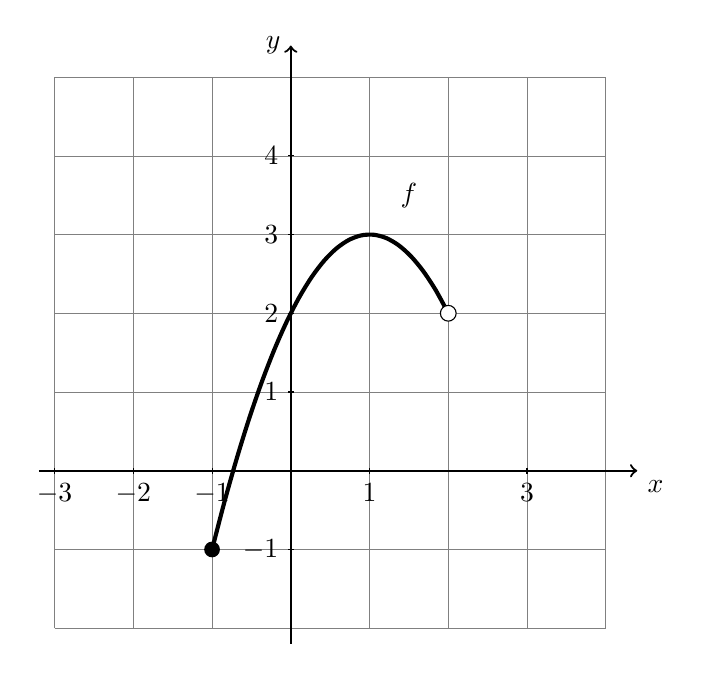
\begin{tikzpicture}[scale=1]
    \draw [help lines] (-3,-2) grid (4,5);
    \draw [thick, ->] (-3.2,0) -- (4.4,0) node [below right] {$x$};
    \draw [thick, ->] (0,-2.2)--(0,5.4) node [left] {$y$};
    \foreach \x in {-3,-2,-1,1, ..., 4} \draw (\x cm,1pt) -- (\x cm,-1pt) node[anchor=north] {$\x$};
    \foreach \y in {-1,1,2,3,4} \draw (1pt,\y cm) -- (-1pt,\y cm) node[left] {$\y$};
    %\draw [thick] (-2,0) -- (0,4) -- (3,5);
    \draw [line width=1.5pt,smooth,samples=20,domain=-1:2] plot(\x,-\x*\x+2*\x+2);
    \fill (-1,-1) circle[radius=0.1];
    \node at (1.5,3.5){$f$};
    \fill [white] (2,2) circle[radius=0.1];
    \draw (2,2) circle[radius=0.1];
  \end{tikzpicture}
\end{multicols}
\vspace{0.5cm}

\item The cost to rent a car is the function of the distance driven in miles plus a fixed charge. The cost in dollars is shown in the table.
\begin{center}
  \begin{tabular}{|l|r|r|r|r|r|r|}
    \hline
    Miles driven & 0 & 50 & 100 & 150 & 200 & 250\\ 
    \hline 
    Rental cost & 40 & 45 & 50 & 55 & 60 & 65\\ 
    \hline 
  \end{tabular}
\end{center}
\begin{enumerate}[itemsep=1cm]
  \item What is the initial fixed charge?
  \item What would be the cost if the car is driven 150 miles?
  \item If the amount charged was \$45, how many miles must have been driven?
  \item Is the incremental cost per mile driven constant? (Is the function linear?) Explain why or why not in the context of the situation.
\end{enumerate}

\newpage
\item A trainer writes a five-week workout plan for a client. For the leg workout two sets of lunges are required, with the number of reps in each set increasing each week. Let $x$ be the week and the number of reps the function of $x$ shown in the table.
  \begin{center}
      Legs workout - lunges (each side, two sets, twice a week)\\
        Week 1: 6 reps\\
        Week 2: 8 reps\\
        Week 3: 10 reps\\
        Week 4: 12 reps\\
        Week 5: 12 reps
    \end{center}
\begin{enumerate}[itemsep=0.25cm]
  \item How many reps are planned for the fourth week, when $x=4$?
  \item Which week has the fewest reps? \\(express your answer in the form $x=$ a number)
  \item Explain what the ordered pair $(3,10)$ would refer to in this context.\vspace{1cm}
  \item Do the reps increase by a constant amount with each week? Explain. \\(If so, what is the slope, or rate of change?) \vspace{1.5cm}
\end{enumerate}

\item Consider the function $f(x)=12-3x$.
\begin{enumerate}
  \item Write down the independent variable.
  \item Calculate $f(2)$ \vspace{2cm}
  \item Show that $\displaystyle f(\frac{5}{3})= 7$ \vspace{2cm}
  \item There is an $x$ for which $f(x)= -27$. \\ Find this value of $x$.
\end{enumerate} \vspace{2cm}

\newpage
\item Challenge: A group of friends rent a professional grill for a party. The rental charge is given by the formula $C(t) = 150 + 35(t)$ where $C$ is the cost in dollars and $t$ is the amount of time the grill is rented in hours.
\begin{enumerate}[itemsep=2cm]
  \item Find the cost of renting the grill for two hours.
  \item Find $C(4)$.
  \item The friends have a budget of \$325 for the grill rental. Determine the number of hours they can afford.
\end{enumerate} \vspace{3cm}

\subsubsection*{Early finishers}
\item Simplify each expression. (Leave it in radical form, not a decimal.)
\begin{enumerate}
  \begin{multicols}{2}
  \item   $\sqrt{18}$ \vspace{1.5cm}
  \item   $\sqrt{48}$ \vspace{1.5cm}
  \end{multicols}
\end{enumerate}
\vspace{2cm}

\item Simplify these fractions problems without a calculator. Show the steps you took.
  \begin{multicols}{2}
    \begin{enumerate}
      \item   $\displaystyle \frac{1}{2} - \frac{1}{3}=$ \vspace{6cm}
      \item   $\displaystyle \frac{2}{5}x+\frac{1}{10}x+\frac{1}{5}=$  \vspace{6cm}
    \end{enumerate}
  \end{multicols}

\end{enumerate}
\end{document}